\chapter{Conclusiones}

\section{Conclusiones Generales}
    
    Esta práctica ha sido la más díficil que hemos realizado, no por el hecho de la dificultad de los algoritmos, más bien por el análisis a posteriori. Encontramos dificultades a la hora de introducir los números necesarios para poder expresar bien el potencial del algoritmo. 
    
    Fuera de esos problemas, encontramos fortalezas a la hora de poder crear algoritmos recursivos y las maneras en que podemos abordar la complejidad de un algoritmo.

\newpage
\section{Isaac Sánchez - Conclusiones}
    Agradezco poder incrementar mis habilidades dentro de los algoritmos recursivos gracias a la practica anterior. Aprendí de mejor manera el análisis a priori de un algoritmo recursivo, acerca de su complejidad y el análisis a priori. Tuvimos complicaciones a la hora de realizar el análisis a posteriori del algoritmo recursivo de la búsqueda de un elemento en un arreglo, esto debido a que desbordaba la memoria dificultando conocer la cantidad adecuada de elementos que debía contener el arreglo.
    \begin{figure}[htp!]
            \centering
            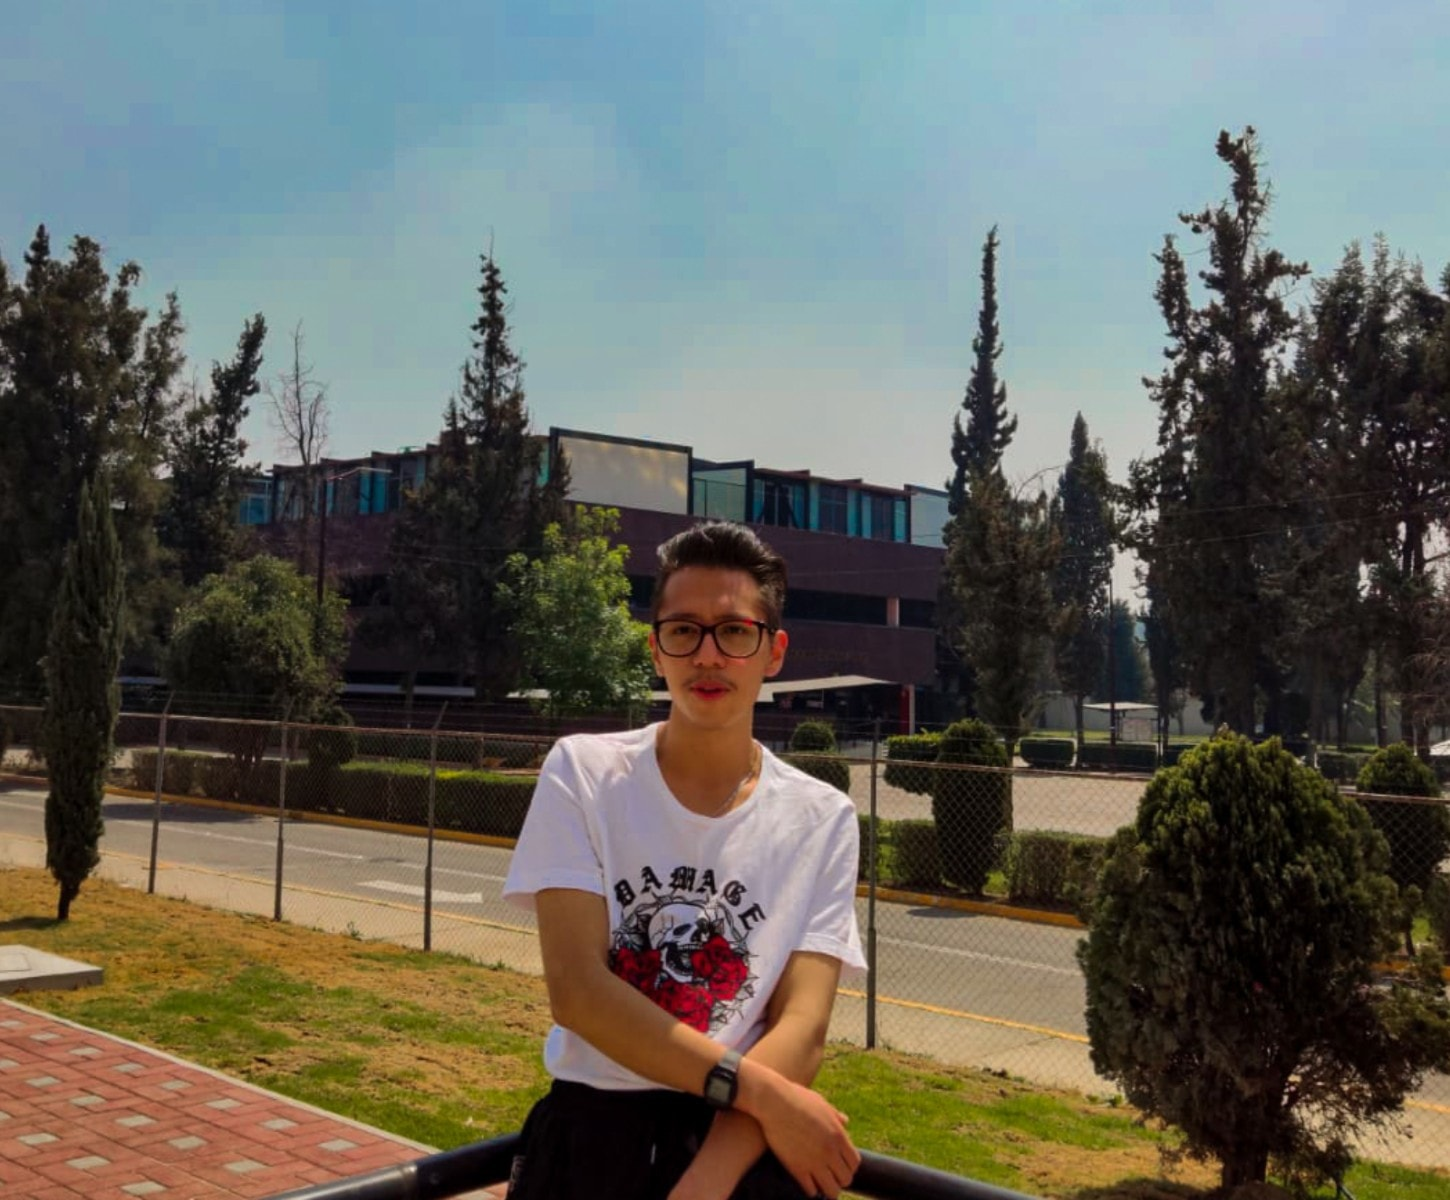
\includegraphics[width=1 \textwidth]{Images/Fotos_Alumnos/274612600_2528992867236334_6677874837890685705_n.jpg}  
            \caption{Isaac Sánchez}
            \label{fig:my_label1}
        \end{figure}
    


\newpage
\section{Axel Trevino - Conclusiones}
    Durante esta práctica se pudo ver la importancia de la recursividad, ya que comparando los algoritmos de ambos ejercicios pudimos visualizar la diferencia de iterativo y recursivo, lo único malo siendo el límite del stack de recursividad
    \begin{figure}[htp!]
            \centering
            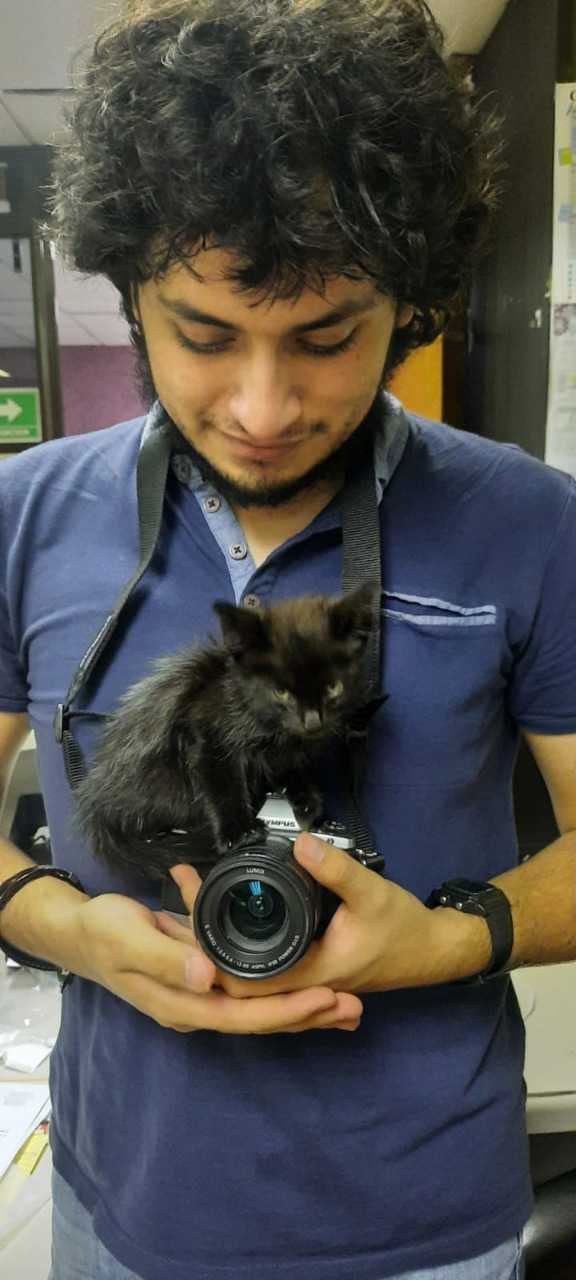
\includegraphics[width=0.4 \textwidth]{Images/Fotos_Alumnos/axel.jpg}  
            \caption{Axel Treviño}
            \label{fig:my_label2}
        \end{figure}
